\documentclass[11pt,a4paper,twoside]{book}
\usepackage[absolute,overlay]{textpos}
\usepackage[top=0.35in,    bottom=0in,    left=0in, right=0in]{geometry}
\usepackage{lipsum}
\usepackage{graphicx}
\usepackage{tcolorbox}
\usepackage{xcolor}

\usepackage{fancyhdr}

\fancypagestyle{pageno}{
	\fancyhf{}
	\fancyfoot[LE]{\raisebox{1.5cm}[0pt][0pt]{\tcbox[colback=blue!48,top=0.15cm, bottom=0.15cm, right=0.6cm, left=0.5cm, boxrule=0mm, arc=0mm]{\textcolor{white}{ \thepage}}}}
	\fancyfoot[RO]{\raisebox{1.5cm}[0pt][0pt]{\tcbox[colback=blue!48,top=0.15cm, bottom=0.15cm, right=0cm, left=0.5cm, boxrule=0mm, arc=0mm]{\textcolor{white}{ \thepage \,\,\,\,\,\,\,\,}}}}
	\renewcommand{\headrulewidth}{0pt}
	\renewcommand{\footrulewidth}{0pt}
}
\pagestyle{pageno}

\fancypagestyle{titlefoot}{
	\fancyfoot[RE]{\raisebox{1.6cm}[0pt][0pt]{\tcbox[colback=white,top=0.15cm, bottom=0.15cm, right=0.6cm, left=0.5cm, boxrule=0mm, arc=0mm]{\textcolor{black}{ Four color theorem}}}}
	\fancyfoot[LO]{\raisebox{1.6cm}[0pt][0pt]{\tcbox[colback=white,top=0.15cm, bottom=0.15cm, right=0cm, left=0.5cm, boxrule=0mm, arc=0mm]{\textcolor{black}{Four color theorem \,\,\,\,\,\,\,\,}}}}
	\renewcommand{\headrulewidth}{0pt}
	\renewcommand{\footrulewidth}{0pt}
}
\pagestyle{titlefoot}

\let\origthepage\thepage
\renewcommand{\thepage}{\fontsize{18}{12}\selectfont\origthepage}

\newenvironment{positionedparagraph}[4]{%
	\begin{textblock*}{#1}(#2,#3)
		\noindent\textbf{#4}\par\medskip
	}{%
	\end{textblock*}
}

\begin{document}
\begin{tcolorbox}[colback=blue!48, colframe=blue!48, width=\linewidth, boxrule=0pt, arc=0pt, outer arc=0pt, sharp corners] \textcolor{white}{\textbf{\\ \\  \Huge Four color theorem \\}}
\end{tcolorbox}

\begin{center}
\tcbox[colback=yellow!20, colframe=yellow!75!black, boxrule=4mm, top=-3 pt, bottom=-3pt, left=38pt, right=38pt, arc=10mm]
{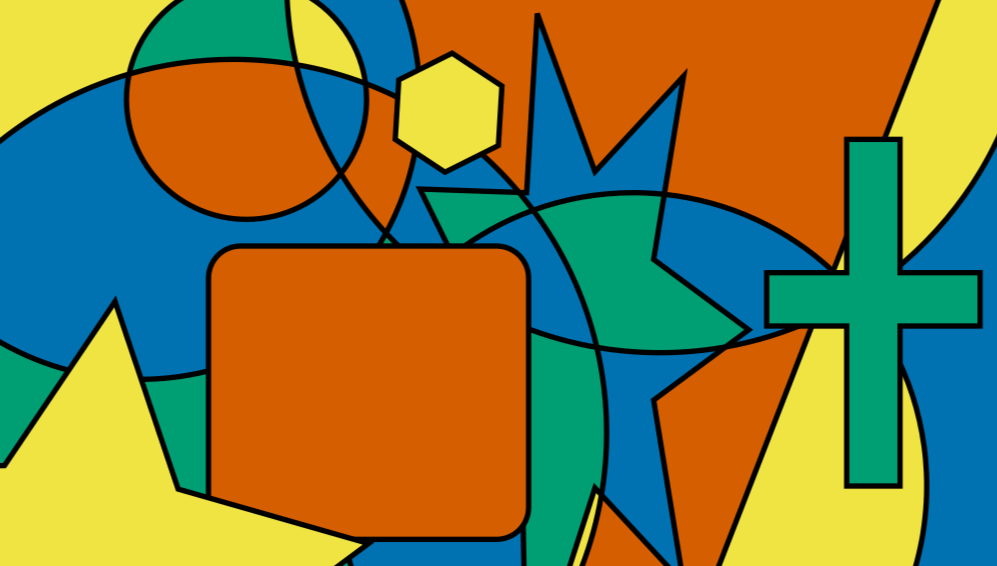
\includegraphics[width=14.5cm]{myimages/pic1.png}}
\end{center}

\begin{positionedparagraph}{0.35\textwidth}{0.07\textwidth}{5.28in}{ \\[-10mm]
\tcbox[colback=blue!48,right=50pt, top=7pt, bottom=7pt, boxrule=0mm, arc=0mm]{\textcolor{white}{\Large Abstract \, \, \, \, \, \, \, \, \,}}}
\noindent This paper is written by \textbf {Devesh Singh \\ Chauhan (I23MA002) }on 18/08/24 as a part of my LaTeX mini project. I don't claim the originality of any of the content mentioned in this paper. Thanks for reading.
\end{positionedparagraph}

\begin{positionedparagraph}{0.42\textwidth}{0.5\textwidth}{5.3in}{ \\[-13.12mm]
\tcbox[colback=blue!48,top=11pt, bottom=11pt, right=100pt, boxrule=0mm, arc=0mm]{\textcolor{white}{\Large Introduction \, \, \,\,\, \,}}}
In mathematics, the four color theorem, or the four color map theorem, states that given any separation of a plane into contiguous regions, producing a figure called a map, no more than four colors are required to color the regions of the map—so that no two adjacent regions have the same color.
\end{positionedparagraph}

\begin{positionedparagraph}{0.83\textwidth}{0.07\textwidth}{18cm}
 \
 For example the image above shows a way in which only four colors are used to fill each "distinct" figure so that no two adjacent figures have the same color coding. The conjecture was first proposed on October 23, 1852 when Francis Guthrie, while trying to color the map of counties of England, noticed that only four different colors were needed.The four color theorem was ultimately proven in 1976 by Kenneth Appel and Wolfgang Haken. It was the first major theorem to be proved using a computer. Appel and Haken's approach started by showing that there is a particular set of 1,936 maps, each of which cannot be part of a smallest-sized counterexample to the four color theorem (i.e., if they did appear, one could make a smaller counter-example).
 
 In graph-theoretic terms, the theorem states that for loopless planar graph G, its chromatic number is x(G) $\le 4$
 First, regions are adjacent if they share a boundary segment; two regions that share only isolated boundary points are not considered adjacent. Second, bizarre regions, such as those with finite area but infinitely long perimeter, are not allowed; maps with such regions can require more than four colors.[4] (To be safe, we can restrict to regions whose boundaries consist of finitely many straight line segments. It is allowed that a region has enclaves, that is it entirely surrounds one or more other regions.) Note that the notion of "contiguous region" (technically: connected open subset of the plane) is not the same as that of a "country" on regular maps, since countries need not be contiguous (they may have exclaves; e.g., the Cabinda Province as part of Angola, Nakhchivan as part of Azerbaijan, Kaliningrad as part of Russia, France with its overseas territories, and Alaska as part of the United States are not contiguous). If we required the entire territory of a country to receive the same color, then four colors are not always sufficient.
\end{positionedparagraph}

\newpage

\begin{tcolorbox}[colback=blue!48, colframe=blue!48, width=\linewidth, boxrule=0pt, arc=0pt, outer arc=0pt, sharp corners]\textcolor{white}{\textbf{\\ \\  \Huge History \\}}
\end{tcolorbox}

\begin{center}
\vspace{0.5cm}
\begin{tcolorbox}[colback=blue!48, colframe=blue!48, width=16cm, top=-0.3cm, bottom=-0.2cm, boxrule=0pt, arc=0pt, outer arc=0pt, sharp corners]\textcolor{white}{\textbf{\\ \\  Early proof attempts \\}}
\end{tcolorbox}
\end{center}
\begin{positionedparagraph}{16cm}{2.55cm}{4.75cm}
	\\ As far as is known, the conjecture was first proposed on October 23, 1852, when Francis Guthrie, while trying to color the map of counties of England, noticed that only four different colors were needed. At the time, Guthrie's brother, Frederick, was a student of Augustus De Morgan (the former advisor of Francis) at University College London. Francis inquired with Frederick regarding it, who then took it to De Morgan (Francis Guthrie graduated later in 1852, and later became a professor of mathematics in South Africa). According to De Morgan:
	
	A student of mine [Guthrie] asked me to day to give him a reason for a fact which I did not know was a fact—and do not yet. He says that if a figure be any how divided and the compartments differently colored so that figures with any portion of common boundary line are differently colored—four colors may be wanted but not more—the following is his case in which four colors are wanted. Query cannot a necessity for five or more be invented
	
\end{positionedparagraph}
\begin{center}
	\vspace{5cm}
	\begin{tcolorbox}[colback=blue!48, colframe=blue!48, width=16cm, top=-0.3cm, bottom=-0.2cm, boxrule=0pt, arc=0pt, outer arc=0pt, sharp corners]\textcolor{white}{\textbf{\\ \\  Proof by computer \\}}
	\end{tcolorbox}
\end{center}
\begin{positionedparagraph}{16cm}{2.55cm}{11.6cm}
	\\ During the 1960s and 1970s, German mathematician Heinrich Heesch developed methods of using computers to search for a proof. Notably he was the first to use discharging for proving the theorem, which turned out to be important in the unavoidability portion of the subsequent Appel–Haken proof. He also expanded on the concept of reducibility and, along with Ken Durre, developed a computer test for it. Unfortunately, at this critical juncture, he was unable to procure the necessary supercomputer time to continue his work.
	
	Others took up his methods, including his computer-assisted approach. While other teams of mathematicians were racing to complete proofs, Kenneth Appel and Wolfgang Haken at the University of Illinois announced, on June 21, 1976, that they had proved the theorem. They were assisted in some algorithmic work by John A. Koch.
	
	If the four-color conjecture were false, there would be at least one map with the smallest possible number of regions that requires five colors. The proof showed that such a minimal counterexample cannot exist, through the use of two technical concepts.
	

	
\end{positionedparagraph}

\begin{center}
\vspace{6.3cm}
\begin{tcolorbox}[colback=blue!48, colframe=blue!48, width=16cm, top=-0.3cm, bottom=0.2cm, boxrule=0pt, arc=0pt, outer arc=0pt, sharp corners]\textcolor{white}{\textbf{\\ \\  Simplification and verification \\[0.2cm]  \footnotesize Since 2005, it is only necessary to trust the Coq kernel\\[-0.3cm]}}
\end{tcolorbox}
\end{center}
\begin{positionedparagraph}{16cm}{2.55cm}{20.45cm}
\\ Since the proving of the theorem, a new approach has led to both a shorter proof and a more efficient algorithm for 4-coloring maps. In 1996, Neil Robertson, Daniel P. Sanders, Paul Seymour, and Robin Thomas created a quadratic-time algorithm (requiring only O(n2) time, where n is the number of vertices), improving on a quartic-time algorithm based on Appel and Haken's proof.[25] The new proof, based on the same ideas, is similar to Appel and Haken's but more efficient because it reduces the complexity of the problem and requires checking only 633 reducible configurations. Both the unavoidability and reducibility parts of this new proof must be executed by a computer and are impractical to check by hand.[26] In 2001, the same authors announced an alternative proof, by proving the snark conjecture.[27] This proof remains unpublished, however. 

\end{positionedparagraph}

\newpage

\begin{tcolorbox}[colback=blue!48, colframe=blue!48, width=\linewidth, boxrule=0pt, arc=0pt, outer arc=0pt, sharp corners] \textcolor{white}{\textbf{\\ \\  \Huge Summary of proof ideas \\}}
\end{tcolorbox}
\begin{positionedparagraph}{18.7cm}{1.2cm}{4.3cm}
\Huge\noindent{{\textbf{\Large Every Planar Map is Four Colorable (Appel \& Haken 1989) }}} \\[0.2cm]
Although flawed, Kempe's original purported proof of the four color theorem provided some of the basic tools later used to prove it. The explanation here is reworded in terms of the modern graph theory formulation above.

Kempe's argument goes as follows. First, if planar regions separated by the graph are not triangulated (i.e., do not have exactly three edges in their boundaries), we can add edges without introducing new vertices in order to make every region triangular, including the unbounded outer region. If this triangulated graph is colorable using four colors or fewer, so is the original graph since the same coloring is valid if edges are removed. So it suffices to prove the four color theorem for triangulated graphs to prove it for all planar graphs, and without loss of generality we assume the graph is triangulated. 
\end{positionedparagraph}

\vspace{5.7cm}
	\begin{figure}[htbp]
	\centering
	\begin{minipage}{0.35\textwidth}
		\centering
		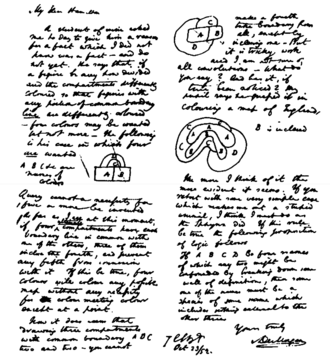
\includegraphics[width=3.5cm]{myimages/pic2.png}
	\end{minipage}
	\hspace{-0.5cm}
	\begin{minipage}{0.25\textwidth}
		\centering
		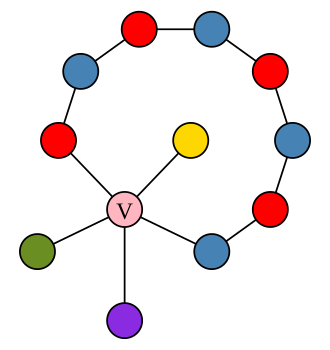
\includegraphics[width=3.5cm]{myimages/pic3.png}
	\end{minipage}
	\hspace{-0.5cm}
	\begin{minipage}{0.35\textwidth}
		\centering
		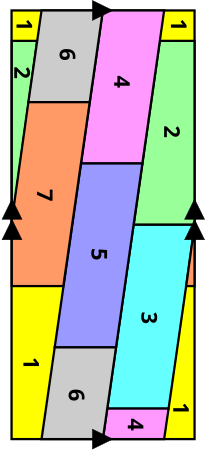
\includegraphics[width=2.2cm]{myimages/pic4.png}
	\end{minipage}
\end{figure}
\begin{positionedparagraph}{18.7cm}{1.2cm}{14.8cm}
\
Suppose \( v \), \( e \), and \( f \) are the number of vertices, edges, and regions (faces). Since each region is triangular and each edge is shared by two regions, we have that \( 2e = 3f \). This, together with Euler's formula, \( v - e + f = 2 \), can be used to show that \( 6v - 2e = 12 \). Now, the degree of a vertex is the number of edges abutting it. If \( v_n \) is the number of vertices of degree \( n \) and \( D \) is the maximum degree of any vertex, ...\\
\[
6v - 2e = 6 \sum_{i=1}^{D} v_i - \sum_{i=1}^{D} i v_i = \sum_{i=1}^{D} (6 - i) v_i = 12.
\]
But since \( 12 > 0 \) and \( 6 - i \leq 0 \) for all \( i \geq 6 \), this demonstrates that there is at least one vertex of degree 5 or less.
If there is a graph requiring 5 colors, then there is a minimal such graph, where removing any vertex makes it four-colorable. Call this graph \( G \). Then \( G \) cannot have a vertex of degree 3 or less, because if \( d(v) \leq 3 \), we can remove \( v \) from \( G \), four-color the smaller graph, then add back \( v \) and extend the four-coloring to it by choosing a color different from its neighbors.


\end{positionedparagraph}

\vspace{6.cm}
\begin{figure}[htbp]
	\centering
	\begin{minipage}{0.45\textwidth}
		\centering
		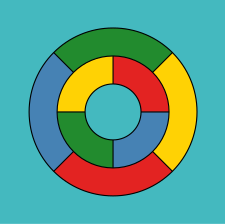
\includegraphics[width=4cm]{myimages/pic5.png}
	\end{minipage}
	\hspace{-2cm}
	\begin{minipage}{0.45\textwidth}
		\centering
		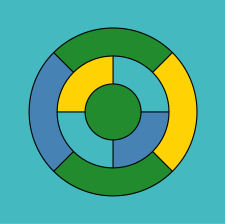
\includegraphics[width=4cm]{myimages/pic6.png}
	\end{minipage}
\end{figure}

\begin{positionedparagraph}{18.7cm}{1.2cm}{25.5cm}
	\
	As long as some member of the unavoidable set is not reducible, the discharging procedure is modified to eliminate it (while introducing other configurations). Appel and Haken's final discharging procedure was extremely complex and, together with a description of the resulting unavoidable configuration set, filled a 400-page volume, but the configurations it generated could be checked mechanically to be reducible. Verifying the volume describing the unavoidable configuration set itself was done by peer review over a period of several years. .  
\end{positionedparagraph}

\newpage
\begin{positionedparagraph}{12.7cm}{1.2cm}{0.5cm}
	\\
	\noindent{{\textbf{\Large False disproofs}}} \\[0.2cm]
	The four color theorem has been notorious for attracting a large number of false proofs and disproofs in its long history. At first, The New York Times refused, as a matter of policy, to report on the Appel–Haken proof, fearing that the proof would be shown false like the ones before it. Some alleged proofs, like Kempe's and Tait's mentioned above, stood under public scrutiny for over a decade before they were refuted. But many more, authored by amateurs, were never published at all. Generally, the simplest, though invalid, counterexamples attempt to create one region which touches all other regions. This forces the remaining regions to be colored with only three colors. Because the four color theorem is true, this is always possible; however, because the person drawing the map is focused on the one large region, they fail to notice that the remaining regions can in fact be colored with three colors. 
\end{positionedparagraph}
\begin{figure}[htbp]
	\vspace{2cm}
	\hspace{15cm}
	\begin{minipage}{0.45\textwidth}
		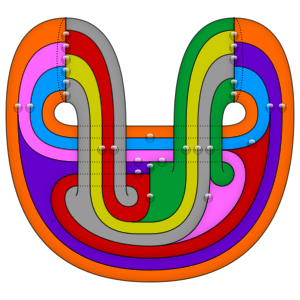
\includegraphics[width=4.1cm]{myimages/pic7.png}
	\end{minipage}
\end{figure}

\begin{figure}[htbp]
	\vspace{1.5cm}
	\hspace{1cm}
	\begin{minipage}{0.45\textwidth}
		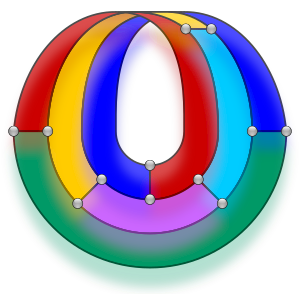
\includegraphics[width=4.1cm]{myimages/pic8.png}
	\end{minipage}
\end{figure}
\begin{positionedparagraph}{13.5cm}{6.2cm}{8.5cm}
	\
	\noindent
	This trick can be generalized: there are many maps where if the colors of some regions are selected beforehand, it becomes impossible to color the remaining regions without exceeding four colors. A casual verifier of the counterexample may not think to change the colors of these regions, so that the counterexample will appear as though it is valid.Perhaps one effect underlying this common misconception is the fact that the color restriction is not transitive: a region only has to be colored differently from regions it touches directly, not regions touching regions that it touches. If this were the restriction, planar graphs would require arbitrarily large numbers of colors. Other false disproofs violate the assumptions of the theorem, such as using a region that consists of multiple disconnected parts, or disallowing regions of the same color from touching at a point. 
\end{positionedparagraph}
\begin{positionedparagraph}{18.7cm}{1.2cm}{14cm}
	\
	\noindent
	The four color theorem applies not only to finite planar graphs, but also to infinite graphs that can be drawn without crossings in the plane, and even more generally to infinite graphs (possibly with an uncountable number of vertices) for which every finite subgraph is planar. 
	\newline\\[-0.3cm]
	To prove this, one can combine a proof of the theorem for finite planar graphs with the De Bruijn–Erdős theorem stating that, if every finite subgraph of an infinite graph is k-colorable, then the whole graph is also k-colorable Nash-Williams (1967). This can also be seen as an immediate consequence of Kurt Gödel's compactness theorem for first-order logic, simply by expressing the colorability of an infinite graph with a set of logical formulae.
\end{positionedparagraph}

\vspace{3.8cm}
\begin{table}[h]
	\centering
	\begin{tabular}{|p{2cm}|p{14cm}|p{2cm}|}
		\hline
		\multicolumn{1}{|c|}{Date} & \multicolumn{1}{c}{Discovery} & \multicolumn{1}{|c|}{Credits} \\
		\hline
		1852 &  first conjectured the Four Color Theorem while trying to color the map of England & Francis\\
		\hline
		1852 & was the first to communicate the problem to the wider mathematical community & Augustu \\
		\hline
		1879 & published what he thought was a proof of the Four Color Theorem  & Kempe \\
		\hline
		1890 & identified the error in Kempe's proof in 1890 but salvaged part of the argument, proving the weaker Five Color Theorem & Heawood \\
		\hline
		1960 & developed the idea of "discharging" and "reducibility," which were crucial for the final computer-assisted proof of the Four Color Theorem. & Heesch \\
		\hline
		1976 & were the first to provide a rigorous proof of the Four Color Theorem & Appel and Haken \\
		\hline
		1976 & published a popular account of the Four Color Theorem & Wilson \\
		\hline
	\end{tabular}
	
\end{table}

\end{document}